\chapter{Neural Network-Based Segmentation of Biomedical Images}
\label{chap:seg-background}

This chapter introduces biomedical images as well as the process of segmenting them. We will start with a brief overview of the most common types of biomedical images.

Biomedical images are a broad and diverse category of images referring to imaging use for the purposes of biology or medicine. These can range from complex modalities such as CT scans all the way to photographs (such as clinical images or photographs of plants). With such a diverse set of modalities and imaging techniques, biomedical images have a low level of cross-domain consistency. Methods developed for one modality often cannot be used in a different modality without modification. This is especially true for learned models such as neural networks. Biomedical image segmentation networks are notoriously bad at out-of-sample performance, i.e. when evaluated on a different modality than they were trained on. This chapter presents a brief overview of various biomedical imaging modalities and techniques, with a focus on those relevant to the methods presented in this thesis.

\section{Common Types of Biomedical Images}

Broadly, we may classify biomedical images into 3D and 2D images. 3D images include modalities such as CT and MRI, but also some types of microscopy as well as other techniques. 2D images, among others, include X-rays, most microscopic images, and dermatoscopic images. The images could also be classified by color space. Techniques that visualize the insides of objects such as CT, MRI or X-ray are usually grayscale. On the other hand, camera-based imaging techniques such as dermoscopy or photographs use three or more color channels. As is apparent, biomedical images do not yield themselves to clean classification, so the classification here is only a general descriptive categorization. There are novel techniques that combine different modalities that escape this classification.

\subsection{3D Modalities}

In medicine, 3D imaging of the patient allows experts to look below the patient's skin. It is hard to overstate the importance of modalities such as CT and MRI on modern medical developments and patient outcomes. These modalities are often captured and stored as voxel-based 3D files, where a voxel is the smallest 3D unit equivalent to a pixel in 3D. They are usually stored alongside patient data such as age, sex, imaging parameters and other relevant information.

\subsubsection{Computed Tomography (CT)}

Computed tomography is an x-ray-based imaging technique where different planes of the subject are captured and then reconstructed into a 3D image using a process called tomography. CT, as opposed to MRI, uses ionizing radiation that can be harmful in large doses. This makes it important to evaluate the cost and benefit of each scan since each scan presents a risk of harming the subject. In addition, image quality is correlated with radiation dose, and the dose is carefully selected based on the required level of image quality so as to not unnecessarily radiate the subject.

Low-dose and high-dose CT images differ enough to cause issues in the segmentation model's performance across these two domains \todo{cite}. High-quality images result in better neural network models, but their availability is much more limited than low-dose scans.

CT can be enhanced using a contrast agent. The contrast agent is usually injected intravenously and is chosen to appear with a high intensity on the resulting image. This makes it easier to delineate blood vessels from surrounding tissue, as is the case e.g. in angiography (CTA).

In the image itself, the values of a CT scan are usually stored as $W \times H \times D$ values, where $W$, $H$, and $D$ are the x, y, and z dimensions, respectively. Each value represents a voxel, \textit{volumetric pixel}, in a 3D volume. The voxels are usually not cubes and can have different lengths along each dimension. In the z-axis, the voxel length is known as slice thickness, and it is chosen based on the task at hand. Thinner slices increase the spatial detail in the image, leading to more details in small tissues. However, thinner slices generally also increase the level of noise in the image, so slice thickness is selected to maintain a tradeoff between spatial resolution and level of noise. The resolution along the x- and y-axes is governed by the field of view and the scanner itself.

The values of the voxels are usually stored as 12 bit signed integer values. The value corresponds to the attenuation of the X-ray as it passes through the tissue. Denser structures such as bones attenuate the radiation more strongly than adipose tissue, and thus result in higher values. This results in higher-intensity voxels in the resulting CT image. To maintain consistency across scans and machines, the attenuation values are linearly transformed such that air has a value of -1000 while water has a value of 0 at standard pressure temperature, as:

\begin{equation}
	{\operatorname{HU}(\mu)}=1000 \cdot {\frac {\mu -\mu _{\textrm {water}}}{\mu _{\textrm {water}}-\mu _{\textrm {air}}}}
\end{equation}

where $\mu$ is the attenuation value of a voxel, and $\mu _{\textrm {water}}$ and $\mu _{\textrm {air}}$ are attenuation values of water and air, respectively. This transformation is called the Hounsfield unit (HU) scale. When calibrated in this way, the attenuation of each tissue is represented as relative to the attenuation of water, and thus values are standardized across images, CT machines, imaging parameters, and centers. Various tissues broadly fall into Hounsfield unit values as is shown in \tabref{tab:hu-tissues}.

\begin{table}[h!]
\centering
\begin{tabular}{l l} 
 \hline
 \textbf{Tissue} & \textbf{Hounsfield value} \\
 \hline
 Fat & -30 to -70 HU\\
 Muscle & 20 to 40 HU\\
 Bone & 1000 HU \\
 Blood & 13 to 50 HU\\
 \hline
\end{tabular}
\caption{Approximate Hounsfield values of various tissues \cite{fosbinder2011essentials, kamalianComputedTomographyImaging2016}.}
\label{tab:hu-tissues}
\end{table}

Hounsfield values are a crucial tool in analyzing medical images. Aside from getting a better understanding of what tissues or objects are present, measured Hounsfield values can have diagnostic significance. For instance, clotted blood has a higher HU value than unclotted blood, and so the Hounsfield value is used as an indicator of intracranial hemorrhage \cite{kamalianComputedTomographyImaging2016}. Another example is using the average HU value of epicardial fat as a sign of myocardial infarction \cite{mahabadiCardiacComputedTomographyderived2017}.

Since the human eye recognizes much fewer gray levels than are available on a CT scan, the scan is typically windowed when viewed by an expert. Windowing refers to the process of shrinking the value range using two thresholds ($t_1$, $t_2$) as:

\begin{equation}
y(x) = 
    \begin{cases}
        t_1, & \text{if } x \leq t_1\\
        x, & \text{if } t_1 < x < t_2\\
        	t_2, & \text{if } x \geq t_2\\
    \end{cases}
\end{equation}

where $x$ is a given HU value. This allows the software to visually stretch the remaining range of gray values to more easily see smaller differences in attenuation, as seen in \figref{fig:windowing-example}. This technique is not limited to human experts. It is common to window CT image inputs into segmentation neural networks. For instance, if segmenting fat, it is often beneficial to discard all voxels outside of the fat tissue range \cite{bencevicRecentProgressEpicardial2022}.

\begin{figure}[h]
 \centering
 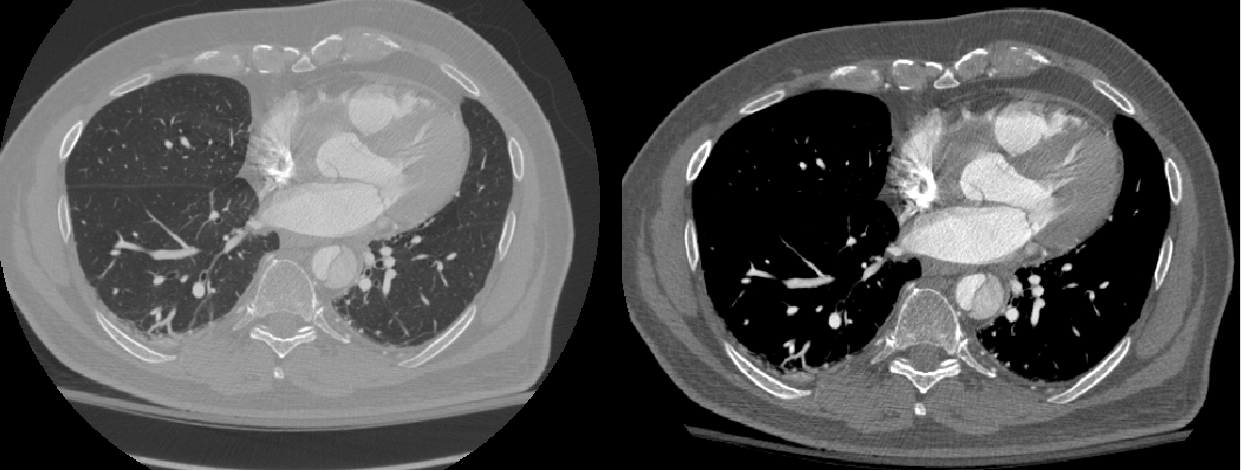
\includegraphics[width=\linewidth]{images/windowing-example}
 \caption{A cardiac CTA in its full range (left) and windowed (right). \cite{radlAVTMulticenterAortic2022a}}
 \label{fig:windowing-example}
 \end{figure}

\subsubsection{Magnetic Resonance Imaging (MRI)}

Much like CT, MRI visualizes the insides of an object using a voxel-based image. MRI works by first applying a strong magnetic field such that protons align parallel to the z-axis. The protons are then excited using a radio frequency pulse which causes them to become misaligned. After the pulse, the protons gradually return back to alignment and induce an electric current. Unlike CT which measures the attention of X-rays, MRI measures this induced current while protons are returning to equilibrium alignment. The time to reach the equilibrium state depends on the specific tissue type. The use of magnetic fields instead of ionizing radiation means that MRI does not cause harm to the patient due to radiation. Unlike CT, MRI values are not standardized across scans and MRI machines, and the specific values can not be used diagnostically across scans, only in relation to surrounding tissues.

MRI generally provides a better contrast than CT, especially in soft tissues. This makes MRI the gold standard of imaging for a large number of tissues and diagnostic procedures. Much like CT, this contrast can be further enhanced using contrast agents. However, MRI imaging is slower when compared to CT which causes patient discomfort, especially for claustrophobic and non-neurotypical patients. MRIs are also not possible in cases where the subject has non-removable magnetic objects such as coronary pacemakers and other implants.

The voxels in an MRI, much like a CT, are generally rectangular solids and can different in the x-, y- and z-axis lengths. The resolution is government by the field of view, the MRI scanner as well as imaging parameters. Generally, increasing resolution leads to higher levels of noise and a longer acquisition time. Thus, a compromise needs to be determined for each imaged tissue and diagnostic task. 

The voxel values are weighted based on the time to reach the equilibrium state which is achieved through two independent processes called T1 and T2. T1 measures the time it takes the protons to reach equilibrium longitudinal magnetization, while T2 measures the time to regain its equilibrium transverse magnetization. Different tissues regain equilibrium states in T2 and T2 at different rates, so MRI images can be weighted according to T1 or T2 time. Water has a long T1 time while fat has a short T1 time, so in T1-weighted images fat appears with a higher intensity than water. On the other hand, water has a high T2 and appears as high-intensity on T2-weighted images. This can be seen in \figref{fig:t1-t2-example}.

\begin{figure}[h]
 \centering
 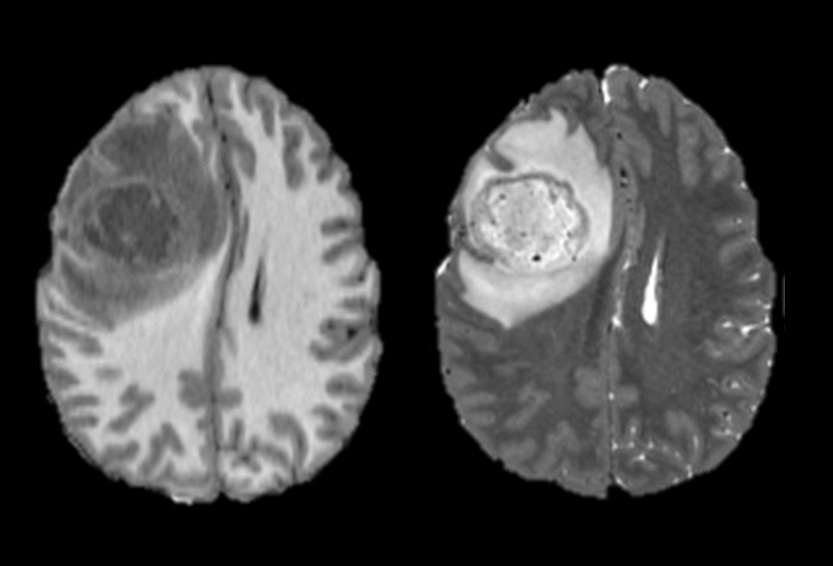
\includegraphics[width=0.65\linewidth]{images/mri-t1-t2-example}
 \caption{An example T1-weighted MRI (left) and a T2-weighted MRI (right) showing a diffuse glioma. \cite{calabreseUniversityCaliforniaSan2022}}
 \label{fig:t1-t2-example}
 \end{figure}

The relative differences in T1 and T2 images make the two weightings more or less beneficial for imaging certain tissues. T1 weighting is useful, among others, for identifying fatty tissue or detecting liver lesions. T2 weighting is useful, among others, for identifying white matter lesions or edemas.

\subsection{2D Modalities}

While 3D modalities offer a detailed view of a subject, they are often time-consuming and invasive in the case of CT. 2D modalities such as X-ray and diagnostic ultrasound are often quicker and more available, making them ideal for screening and simpler diagnostics. The same reason also results in a much larger amount of publicly available datasets in 2D modalities compared to 3D ones. Segmentation, object detection, and classification in X-ray images, for instance, is one of the most active fields in computerized medical image analysis research \cite{nguyen2020vindrcxr, irvinCheXpertLargeChest2019}.

\subsubsection{X-ray imaging}

Similarly to CT, X-ray imaging or radiography uses ionizing radiation emitted on one side of the object and detected on the other. The intensity of the image corresponds to the attenuation of the emitted radiation. Denser materials appear with a higher intensity on the resulting image due to their high attenuation.

When capturing an X-ray image, an expert manually positions the generator. The position of the generator and the object determine the magnification and field of view in the image. If the distance between the detector and the object is larger than the distance between the generator and the object, the object will appear larger on the resulting image. This magnification means that the scale on an X-ray image is relative to the image itself and so objective measurements cannot be made on an X-ray.

The expert also determines various parameters that ultimately change the quality and quantity of the X-ray beams. The quality measures the ability of an X-ray to penetrate tissue and is proportional to the X-ray energy level. Quantity, on the other hand, measures the number of photons that constitute the beam. Increasing the beam quality allows for imaging denser tissues such as bones or through large bodies but results in lower contrast in soft tissues. This means that intensity in X-rays is not standardized across images like it is in CT, and so there is no objective unit of measuring X-ray intensity.

\subsubsection{Dermatological images (clinical and dermatoscopic)}

An increasingly active application of deep learning-based models is in dermatological applications, namely skin lesion analysis. This is driven in part by organisations such as the International Skin Imaging Collaboration (ISIC) that curates large dermatological datasets \cite{rotembergPatientcentricDatasetImages2021}. These datasets consists of clinical and dermatoscopic images. Clinical images are regular photographs of skin lesions, while dermatoscopic images are captured with a digital epiluminescence dermatoscope. This dermatoscope consists of a camera attached to a magnifying lens with a built-in light source. It allows capturing detailed and magnified images of a skin lesion while filtering out skin reflections.

The primary application of deep learning in dermatological images is for classification --- predicting whether a lesion is benign or not or detecting the type of skin disease. However, skin lesion segmentation plays a role in the detection as delineating the skin lesion border can be used to provide more objective attributes of the skin lesion \cite{rotembergPatientcentricDatasetImages2021}.

\subsubsection{Microscopy}

In biomedicine, one of the most used applications of computer vision is in segmenting, analyzing, and quantifying microscopic images. This encompasses various tasks in digital pathology such as detecting cancerous cells, segmenting nuclei, or counting white blood cells.

Publicly available microscopic images of cells are abundant due to how frequently they are captured and that they don't contain any personally identifiable information. However, these images sometimes present a challenge due to their size. Microscopic images can have an area of multiple megapixels, far too large for current deep-learning models. Therefore, the images are often split into patches, downscaled or analyzed in a coarse-to-fine manner \cite{jhaInstanceSegmentationWhole2021a}.

With those modalities in mind, we can now cover the process of segmenting the images.

\section{Image Segmentation: From Images to Segmentation Maps}

Image segmentation is the process of categorizing each pixel (or voxel) of an image as belonging to one of several predefined classes. For instance, a 3-class problem of segmenting CT images could be liver, liver tumour, and background. Each class gets assigned an arbitrary class label, such as `0', `1' and `2' for the background, liver and tumour, respectively. The segmentation output is another image of the same size, only the value for each voxel corresponds to the class label of that voxel. Voxels belonging to the liver would each have a value of `1', etcetera. This resulting image is called a \textbf{segmentation map}, since it acts as a map for the original image. In medical image segmentation commonly only target is segmented, which is called \textbf{binary segmentation} since we are using two classes, the target, and the background.

However, multi-class segmentation problems can be reduced to a set of binary segmentation problems where a separate class-vs-background segmentation map is constructed for each class. Mathematically, given a set of $K$ classes, and an input $d$-dimensional image of $N$ channels $I(A)$, $I \in \mathbb{R}^{N}$, $A \in \mathbb{Z}_{\geq0}^d$ where A is a vector representing the location of each voxel, the segmentation map can be expressed as a function $M : \mathbb{Z}_{\geq0}^d \rightarrow \mathbb{R}^K$ mapping each pixel location to a vector of class probabilities:

\begin{equation}
M(A) = (\;\prg{C_0}{I(A)},\; \prg{C_1}{I(A)},\; \cdots\!,\;  \prg{C_{K - 1}}{I(A)}\;),
\end{equation}

where $\operatorname{Pr} (C_i \!\mid\! I(A))$ denotes the probability that the voxel $I(A)$ contains an object of class $C_i$. Expressed this way, the segmentation map is a $K$-channel image of the same size as $I$, where each channel corresponds to a probability map of finding an object of a given class at a given voxel location. 

In the case of binary segmentation where $C_0$ is the background and the $C_1$ is the target object, $\prg{C_1}{I(A)} = 1 - \prg{C_0}{I(A)}\; \forall A$ and therefore $M(A)$ can be treated as a scalar value $M(A) = \prg{C_1}{I(A)}$. This representation is very common as many medical image segmentation problems are binary segmentation problems, such as segmenting organs, cell nuclei, skin lesions, etc.

Ultimately, to delineate tissues the segmentation masks $M(A)$ are commonly binarized such that voxels containing the target object become `1' and the background becomes `0'. This is why $M(A)$ is also commonly called a \textbf{segmentation mask}. In computer vision, the term mask refers to a binary image $M_{01}(A) \in \{0, 1\}$ that hides (masks) regions in another image producing a masked image $I_m(A) = I(A) M_{01}(A)$. In the context of deep learning-based image segmentation, the terms segmentation map and segmentation mask are often used interchangeably.

What follows is a broad overview of commonly used medical image segmentation methods, from traditional ones based on heuristics to complex model-based approaches broadly used today.

\subsection{Traditional Image Processing Methods}

For the purpose of this review, traditional image processing methods include techniques like thresholding, region growing, active contours, as well as morphological operations. These are often combined with heuristic strategies to refine the segmentation area, establish an initial contour, or enhance advanced methods. Heuristics are best-practice rules derived from previous samples and experiences. For instance, the longest component in the bone intensity range of an X-ray image is usually the femur.

These methods are usually developed with a very specific application in mind and are hard to translate to other tasks and domains without significant changes. They are also sensitive to parameter selection and properties of the image such as intensity level. However, since they don't use a learning component they are easily explainable and their limitations can be known ahead of time. Their validity can also be confirmed using fewer samples than is the case for learning-based methods.

Despite the popularity of deep learning, these techniques still play a vital role in modern medical image segmentation. Traditional techniques are often used as methods for pre-processing and data augmentation, as well as refining deep learning model outputs. As we will show later in the dissertation, this can both increase the robustness and data efficiency of deep learning-based segmentation models.

\subsubsection{Image Thresholding}

As mentioned earlier in this chapter, voxel intensities on CT scans are measured using the Hounsfield scale, which represents the tissue's X-ray radiation attenuation at each pixel. Pixels indicative of adipose tissue usually fall between -250 HU and -30 HU. This range provides a means to segment adipose tissue by applying image thresholding. A large number of studies presenting CT segmentation methods use thresholding, at least partially, to segment an object. Hounsfield unit thresholding is an easy and safe way to discard irrelevant voxels and allow the model to focus on a few number of voxels. 

It can be also used to greatly simplify a model's task. In the case of epicardial fat segmentation, the fatty tissue is sparsely distributed in a complex shape inside the pericardium. However, the pericardium itself has a smooth, elliptical shape and is comparatively easy to segment. By segmenting the pericardium and then thresholding the pericardium region to the fatty tissue range, we can find epicardial fat without having to segment its complex shape directly \cite{bencevicRecentProgressEpicardial2022}.

\subsubsection{Region Growing Techniques}

Region growing is a voxel-based image segmentation method \citep{regionGrowing}. Beginning from a designated seed voxel, the method assesses neighboring pixels in successive steps. If these pixels meet a specified criterion, often related to pixel values or textures, they are integrated into the region. Despite being a straightforward method, region growing's effectiveness relies heavily on the seed point selection and may struggle with nuanced transitions between regions. This process is shown in \figref{fig:region-growing}.

\begin{figure}[h]
 \centering
 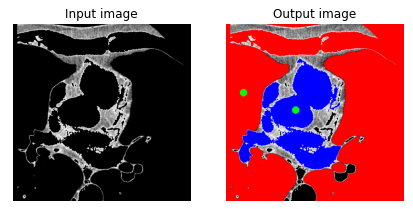
\includegraphics[width=0.7\linewidth]{images/region_growing.png}
 \caption{A demonstration of region growing for delineating the internal and external areas of the pericardium on a CT slice, set to the adipose tissue intensity range. The left image is the original input, and the right image depicts the segmented outcome with the heart exterior in red and the interior in blue. The green dots represent the manually chosen seed points initiating the region-growing technique. \cite{bencevicRecentProgressEpicardial2022}}
 \label{fig:region-growing}
 \end{figure}


\subsubsection{Active Contours or Snakes}

Active contours, often termed "snakes", are segmentation methods that employ dynamic curves to outline image parts \citep{Kass1988}. The process involves tightening a preliminary curve around an object iteratively until it conforms to the object's shape. The adaptation is guided by an energy function that evaluates the curve's smoothness and proximity to edges. A practical depiction of active contours is displayed in \figref{fig:active-contour}.

 \begin{figure}[h]
 \centering
 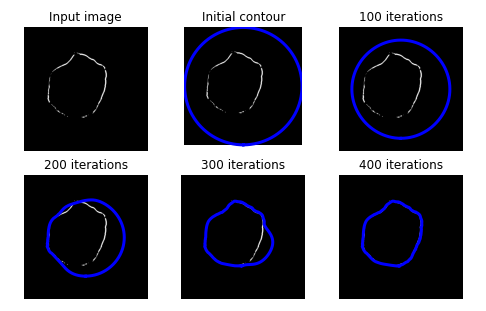
\includegraphics[width=0.65\linewidth]{images/active_contour.png}
 \caption{A demonstration of employing active contours to complete the absent segments of the pericardium line, displayed in white. The contour, illustrated in blue, starts as a complete circle surrounding the image. With every iteration, the contour adapts more closely to the image's shape. \cite{bencevicRecentProgressEpicardial2022}}
 \label{fig:active-contour}
 \end{figure}

\subsubsection{Atlas-Based Segmentation}

Atlas-based methods, differing from contour-based ones, leverage the spatial relationships among structures \citep{Rohlfing2005}. An expert typically creates an atlas by manually segmenting and labeling structures in an image. Due to anatomical variations, multiple atlas images are often merged to produce a representative version. This consolidated atlas can then be employed to segment new images using a registration algorithm. Image registration is an optimization problem where one image, called the moving image, is deformed to best align with a target image according to some scoring function. In atlas-based segmentation, a new moving image is deformed to be aligned with the target image that was used to construct the atlas. The atlas can then be used as a segmentation map for the moving image, as it is now aligned with the atlas. 

The scoring function usually uses the distance between heuristic-based landmarks in the target and moving images to determine how well the two images align. The atlas-based registration process is illustrated in \figref{fig:registration}. A disadvantage of this approach is that the process can lead to a complete failure to segment the image if the target and moving images are too dissimilar.

\begin{figure}[h]
 \centering
 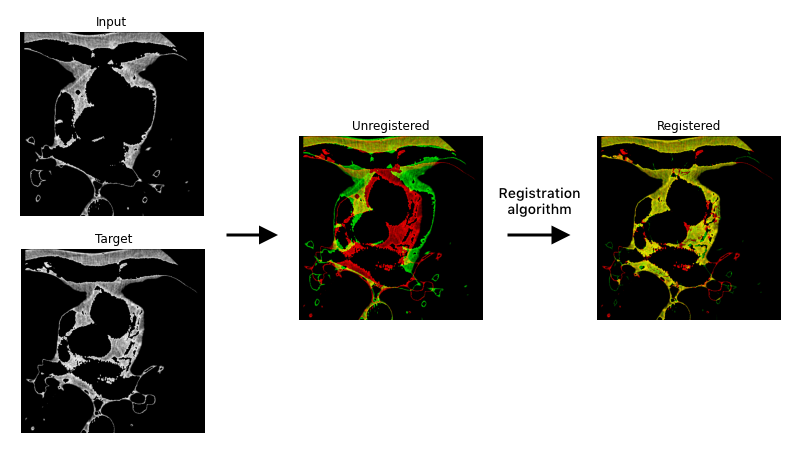
\includegraphics[width=0.7\linewidth]{images/registration.png}
 \caption{A schematic representation of the registration procedure. Initially, input and target images are chosen. Throughout the registration phase, the input image (shown in green) undergoes deformation to align with the fixed target image (shown in red). \cite{bencevicRecentProgressEpicardial2022}}
 \label{fig:registration}
 \end{figure}

Atlas-based segmentation has fallen out of favor due to the emergence of deep learning-based methods. However, recently there has been significant progress in image registration and atlas-based segmentation using deep learning-based techniques \cite{sinclairAtlasISTNJointSegmentation2022a}. These approaches offer good potential for merging traditional and newer approaches will be discussed later in the chapter.

\subsection{Machine Learning}

While deep learning generally falls within the machine learning umbrella term, in this dissertation the term ``machine learning'' will be used to describe techniques that are not based on deep neural networks. These include methods like support vector machines, deep forests or manual feature engineering.

Within this context, it is possible to define a segmentation problem as a per-voxel classification problem. Let there be a classifier of $K$ classes,

\begin{equation}
H(x; \theta) = (\;\operatorname{Pr}(C_0\!\mid\!x),\; \operatorname{Pr}(C_1\!\mid\!x),\; \cdots,\; \operatorname{Pr}(C_{K-1}\!\mid\!x)\;),
\end{equation}

parameterized by $\theta$ with input voxel-level feature vector $x$. The features are manually selected and constructed to represent each pixel and its surrounding region. Commonly, these include the pixel's intensity, mean intensity of the area, image moments, and other information deemed relevant for the classification. The classifier is trained to minimize a loss function by feeding each pixel's features to the classifier and comparing the output to the ground truth output. A visual demonstration of this machine-learning process for image segmentation is shown in \figref{fig:machine-learning}.

\begin{figure}[h]
 \centering
 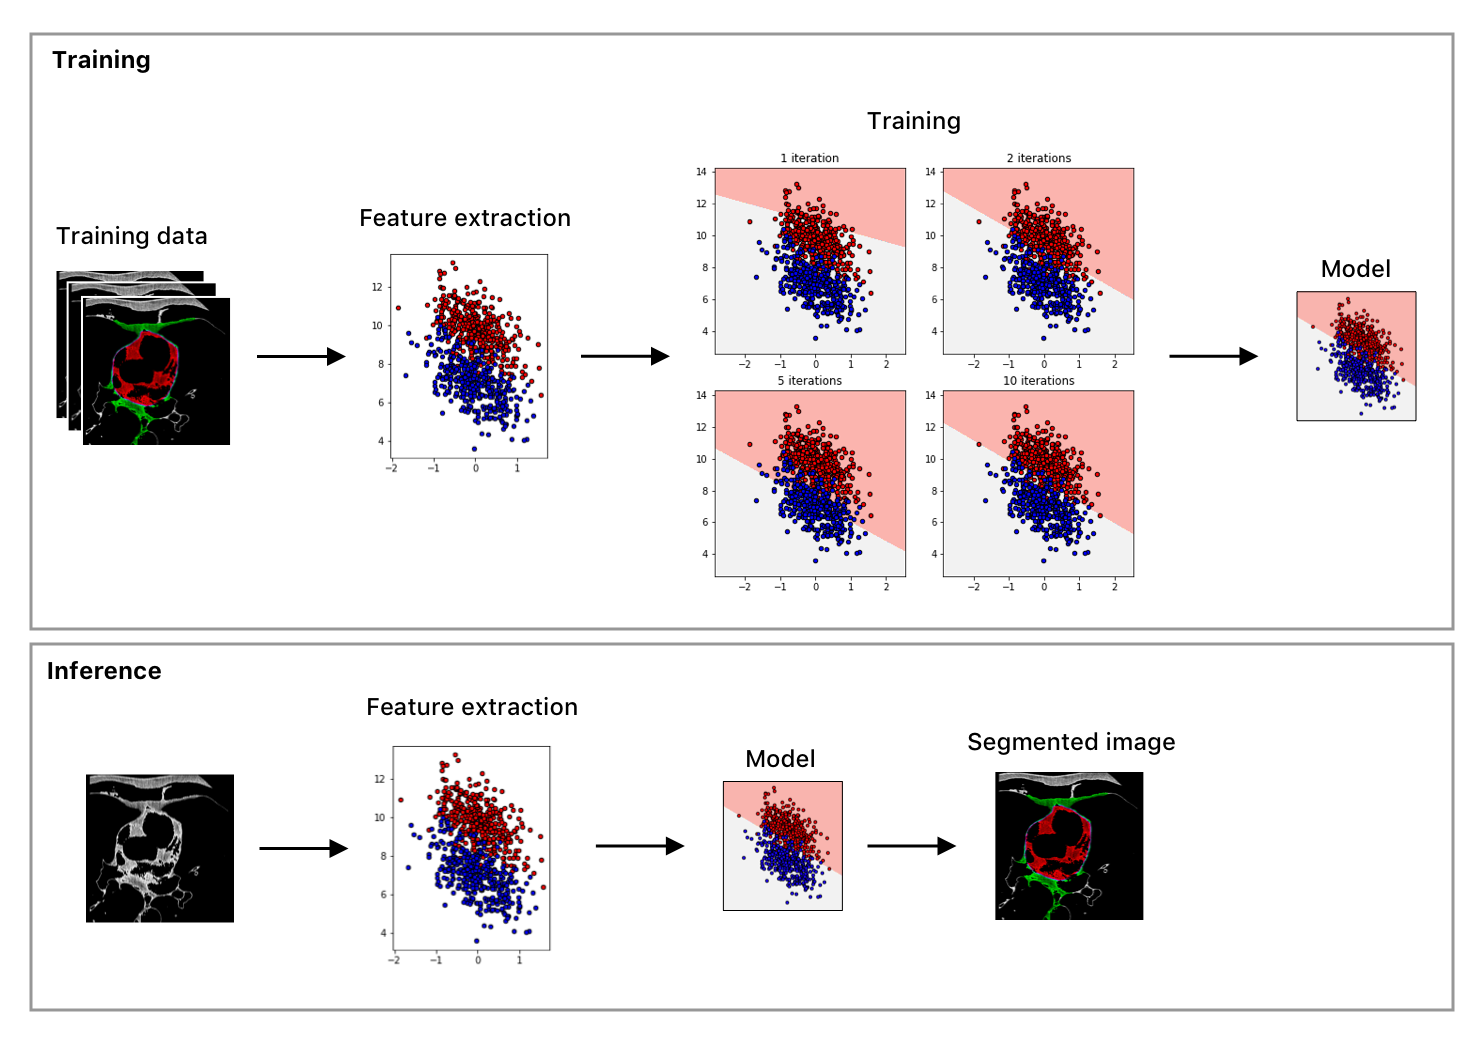
\includegraphics[width=\linewidth]{images/machine_learning.png}
 \caption{A schematic of a supervised linear classifier in a machine learning workflow. The upper section illustrates the training phase. Here, features are color-coded according to their known class from training data, depicted in red and blue. The parameters of the decision boundary, which demarcates the zones of the two classes (highlighted in light red and grey), are determined during training. The lower part of the diagram depicts the inference stage. In this phase, features are extracted from new images, and the trained model is employed to classify each pixel in the image. \cite{bencevicRecentProgressEpicardial2022}}
 \label{fig:machine-learning}
 \end{figure}

Another common approach is splitting the image into smaller patches, and then using a machine learning classifier to class each patch into belonging to one of a set of $K$ classes. The classifications are then fused together to form a segmentation map.

These approaches can be more data efficient than deep learning-based approaches \cite{bencevicRecentProgressEpicardial2022} but have a limited ability to model complex features and dependencies. 

Now that we have an overview of more traditional methods, we can dive into deep learning-based ones.

\section{Deep Learning-Based Segmentation Methods}

While machine learning encompasses a broad range of techniques for building statistical models, deep learning focuses on using artificial neural networks. Artificial neural networks consist of simple nodes called neurons. Each neuron is a non-linear function of the sum of its inputs. This non-linear function is called the \textbf{activation function}. The neurons are all arranged in a graph where the outputs of one set of neurons are connected to the input of another set of neurons. Each connection has an associated \textbf{weight} and \textbf{bias} parameter that either multiplies by the weight or adds the bias value to the output before it goes into the next neuron. The exact configuration of the graph, i.e. the number of neurons and how they are connected, is determined by hand and is referred to as the \textbf{neural network architecture}. A typical neural network architecture can be seen in \figref{fig:nn-typical}.

Typically, neurons are arranged into \textbf{layers}, where neurons of a layer connect only to the next layer, without skipping layers in between. Current deep-learning networks usually have between ten and 100 layers.

As an example of a simple neuron, we can imagine a neuron that receives a 3-valued vector as an input and produces an output using the rectified linear unit (ReLU) function:

\begin{equation}
ReLU(x) = 
    \begin{cases}
        x, & \text{if } x > 0,\\
        x, & \text{otherwise.}\\
    \end{cases}
\end{equation}

ReLU can be seen as a simple thresholding function that clamps values below zero to zero. In spite of its simplicity, ReLU is one of the most activation functions in neural networks.

First, the input vector $x = [x_0\; x_1\; \cdots\; x_{n - 1}]$ is multiplied by the weights column vector $w$ and added with the bias vector $b$:

\begin{equation}
z(x;w, b) =
\begin{bmatrix}
x_0 & x_1 & \cdots & x_{n - 1}
\end{bmatrix}
\begin{bmatrix}
w_0\\
w_1\\
\cdots\\
w_{n-1}
\end{bmatrix}
+
\begin{bmatrix}
b_0 & b_1 & \cdots & b_{n - 1}
\end{bmatrix}
\end{equation}

Then, all of the inputs are summed and the neuron output is produced using the activation function $af$ (in the case of this example ReLU):

\begin{equation}
f(x;w,b) = af\left(\sum_{i=0}^{n - 1} z(x;w,b)_i\right).
\end{equation}

The parameters $b$ and $w$ of each neuron can be stored inside a large matrix $\theta$. This matrix is called the \textbf{parameters of the network}. Current deep learning networks usually have multiple millions of parameters.

\subsection{Neural Network Training, Validation and Testing}

Initially, the values of these parameters are usually set to random numbers. Their exact values are determined automatically through a process called \textbf{training}. During training, the values of the network's parameters are iteratively adjusted to minimize the value of a \textbf{loss function}. The loss function measures how well the network is performing its task based on known correct values. For instance, in image segmentation, the loss function would measure the similarity between a hand-labeled segmentation map and the one produced by the network. Using a process called backpropagation, each parameter is updated in the direction that will decrease the loss function's value. This is repeated multiple times for each image in a \textbf{training dataset}.

The training dataset, much like any statistical data, is a sampling of the real world. Depending on the size and quality of the dataset, it is possible that the training dataset is not representative of the true distribution of the data. Moreover, it is also possible that the network learns to produce correct solutions for each training image individually instead of learning general patterns in the data. This is called \textbf{overfitting} --- the network learns to minimize the loss in the training data but does not generalize to data outside the training domain. To overcome this, two other datasets are used besides the training dataset.

The \textbf{validation dataset} is used to assess the model's performance during model development. While creating a model, one has to make decisions about the architecture, data processing, and other implementation details. To evaluate these decisions, inference is performed on the validation dataset (with known correct values) to estimate its real-world performance. However, the network is never trained on the validation dataset, it is only validated after the training process. The third \textbf{test dataset} (sometimes called a hold-out dataset) is used only once the development process is completed as a final estimate of real-world performance.

The training, validation, and testing datasets are created before the model development process. Usually, they are sampled randomly from a larger dataset with ratios such as 80\%, 10\% and 10\% for the training, validation, and testing datasets, respectively. In the next chapter, we will discuss overfitting in more detail.

\subsection{Encoders and Decoders}

Machine and deep learning-based segmentation methods can be framed as consisting of two stages:

The first stage is an \textbf{encoder} stage $En : \mathbb{R}^{W \times H \times C} \rightarrow \mathbb{R}^{n \times m \times d}$ which maps an image of size $W \times H$ and $C$ channels into a feature vector. This stage can be seen as encoding salient information in the image in a smaller representation, effectively compressing the image --- leading to the name encoder. In deep learning parlance sometimes this is referred to as the \textbf{backbone} of the network.

The output of the encoder is given to the second stage called the \textbf{decoder} or the \textbf{segmentation head}. The decoder is a function $De : \mathbb{R}^{n \times m \times d} \rightarrow \mathbb{R}^K$ that maps a given feature map into a segmentation map. Given an image $I(A)$, the segmentation process can then be written as:

\begin{equation}
M(A) = (En \circ De)(I(A))
\end{equation}

$En$ is a function parameterized by a vector of parameters $\theta_{En}$, while $De$ is parameterized by $\theta_{De}$. In machine learning approaches, $En$ is not a trainable function and $\theta_{En}$ consists of hand-selected parameters such that it extracts pre-selected features from the image. The value of $\theta_{De}$, on the other hand, is determined by minimizing a loss function. The loss function measures how well the model segments an image compared to a ground truth known segmentation of that same image. However, in deep learning approaches, both $\theta_{En}$ and $\theta_{De}$ are determined by minimizing a loss function.

Thus, the difference between traditional machine learning and deep learning is in the encoder stage. In deep learning, the values of the features are determined by a neural network, while in machine learning they a produced using a hand-crafted function.

The separation of segmentation models into encoder and decoder stages is a crucial aspect of current research in deep learning. This separation allows for independent improvement of both stages and an easy combination of different encoders and decoders. For instance, a classification and segmentation network could use the same encoder architecture. The classification model would use a simpler decoder that maps the input features into a vector of length $K$ representing the score for each of the $K$ classes. The segmentation model would use a comparatively complex backbone that produces a segmentation map. However, both models would use the exact same encoder. In fact, there are models such as Mask R-CNN \cite{heMaskRCNN2018} that use two parallel decoders for different tasks, both connected to the same encoder. Throughout the rest of this thesis, when describing neural network architectures, we will describe them in terms of their encoder and decoder and how the two are connected.

\subsection{Convolutional Neural Networks}

Convolutional neural networks have spurred a revolution in computer vision and made deep learning the de facto standard for solving complex computer vision tasks. The central aspect of a \ac{cnn} is the convolutional layer. The convolutional layer replaces the standard neuron mentioned earlier in this chapter with a convolution-like operation.

Generally, convolution is a mathematical operation between two functions, but for the purposes of this introduction, we will only consider 2D convolutions between two square images, as that is most relevant for image segmentation. Convolution is an operation $I(A) \star k(B)$ where $I(A)$ is an image $I(A) \in \mathbb{R}^{W \times H}$ and $k(B)$ is a matrix $k(B) \in \mathbb{R}^{w \times h}$ indexed by locations $B \in \mathbb{Z}_{\geq0}^2$ for 2-dimensional images. The second matrix is called the \textbf{convolutional kernel}. The convolution operation at $A = (a_x, a_y)$ can then be defined as:

\begin{equation}
(I \star k)(a_x, a_y) = \sum_{j=-\infty}^{\infty} \sum_{i=-\infty}^{\infty} I[i, j] k[a_x - i, a_y - j].
\end{equation}
 
Explained differently, the resulting image is produced by sliding the kernel over the input image, one pixel at a time. At each pixel location, values where the kernel and the image overlap are multiplied, and all of the products are summed together to form the value of that pixel in the resulting image. This is shown visually in \figref{fig:convolution-explanation}.

While mathematically a simple operation, convolution is exceedingly powerful and can produce almost endless transformations of an image. It's most commonly used for filtering: A convolution can elegantly find patterns in the image. One such example is the convolution with a kernel called the Prewitt operator:

\begin{equation}
I_y(A) = I(A) \star \begin{bmatrix}
-1 & 0 & 1\\
-1 & 0 & 1\\
-1 & 0 & 1\\
\end{bmatrix}
\end{equation}

When convolved with this kernel, the resulting image has high-intensity pixels in regions where vertical edges are present, and low intensity everywhere else. This can be seen in \figref{fig:prewitt-example}.



In the image, the values of vertical edges necessarily have to have a large jump in values going from left to right or right to left. Otherwise, there would be no perceptible edge. This kernel takes advantage of that fact to accentuate parts of the image where there is such a jump. It does this by replacing each pixel with the difference between the pixels on its left and its right.

Here is how this happens: for each pixel of the input image, the kernel is placed such that it is centered on that pixel. This means that the values of the pixel as well as its neighbors above and below are all multiplied by zero. The neighbors on the left are multiplied by -1, and the ones on the right are multiplied by 1. Summed together, the result represents the sum of the values on the right of the pixel, minus the sum of the values on the left.

To illustrate this, let us zoom into a region of the image where no vertical edges are present:

\[
\begin{bmatrix}
128 & 130 & 136\\
\end{bmatrix}
\star
\begin{bmatrix}
-1 & 0 & 1\\
-1 & 0 & 1\\
-1 & 0 & 1\\
\end{bmatrix}
=
\sum_{i,j}
\begin{bmatrix}
-1 \times 0 + 0 \times 128 + 1 \times 130\\ 
-1 \times 128 + 0 \times 130 + 1 \times 136\\
-1 \times 130 + 0 \times 136 + 1 \times 0\\
\end{bmatrix}
= 8
\]

This section of the image does not contain a vertical edge, so the convolution result is a relatively low value. In a standard image with values in $[0, 255)$, 8 would appear almost completely black.

However, consider some section of the image where a vertical edge is indeed present:

\[
\begin{bmatrix}
63 & 66 & 132\\
\end{bmatrix}
\star
\begin{bmatrix}
-1 & 0 & 1\\
-1 & 0 & 1\\
-1 & 0 & 1\\
\end{bmatrix}
=
\sum_{i,j}
\begin{bmatrix}
-1 \times 0 + 0 \times 64 + 1 \times 66\\ 
-1 \times 64 + 0 \times 66 + 1 \times 132\\
-1 \times 66 + 0 \times 132 + 1 \times 0\\
\end{bmatrix}
= 68
\]

The value is now much larger due to the difference between the left and right sides of the image.

Aside from edge detection, there are many commonly used convolution kernels to perform common task such as blurring, sharpening, or denoising images. A \ac{cnn} can leverage the power of the convolution by stringing together kernels to match complex and intricate patterns in the image.

In a \ac{cnn}, convolutional layers are connected to one another in a similar fashion to neurons in a regular neural network. One convolutional layer performs a user-defined number of convolutions $n$, and stores the result in an $n$-channeled matrix called a \textbf{feature map} where each channel is a convolution of the input with a new kernel. Thus, a convolutional layer holds $n$ convolutional kernels. The values of the kernels are the parameters of the layer --- i.e. they are set during training to minimize a loss function. Finally, a convolutional layer also has an activation function and it is applied to the resulting feature map. Just like in a regular neural network, this allows non-linear operations between convolutional layers, giving them the ability to find more complex features.

The actual operation inside a convolutional neural network differs from the mathematical convolution we described earlier but achieves a similar effect. Firstly, both the kernel and the image are three-dimensional --- after all, the input image usually has 3 channels, and convolutional layers themselves can have thousands of channels. The kernel is therefore a $w \times h \times c$ matrix. 

In each step, the kernel volume slides across the spatial (width and height) dimensions of the input, and stretches across the input since it has the same number of channels. Just like in the 2D convolution described above, all of the values are multiplied and the products are summed to produce one scalar value. Thus, the result of each convolution is still two-dimensional, since the kernel only slides along the width and the height of the input. This is visualized in \figref{fig:cnn-conv-explained}.

\begin{figure}[h!]
 \centering
 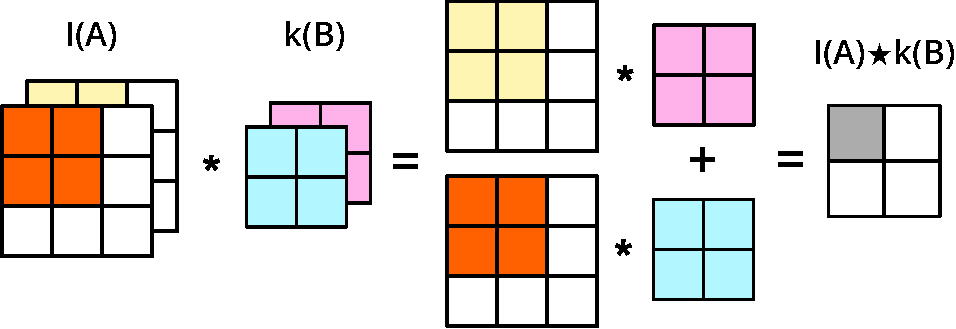
\includegraphics[width=0.8\linewidth]{images/cnn-operation-explained}
 \caption{A view of one step of a single convolution operation inside a \ac{cnn} layer. The layer performs multiple convolutions, each with a different kernel that has an equal number of channels as the input image. In each step, the whole kernel slides over the width and height of the image, and the overlapping channels are multiplied together and summed to produce a single output value. The output of the convolution is one channel of a $n$-channel image where $n$ is the number of different kernels in the layer.}
 \label{fig:cnn-conv-explained}
 \end{figure}

Generally, most \ac{cnn}-based encoders follow a similar pattern of gradually reducing the width and height of the feature maps while increasing their depth. Depth is increased by giving each successive convolutional layer more kernels, thus increasing the output depth since each channel is the output of a convolution using one of the kernels. The spatial (width and height) dimensions are reduced using \textbf{pooling layers}. These layers downsample the image in some way, such as averaging each surrounding neighborhood of pixels. By doing so, a convolutional neural network achieves two goals. First, detailed spatial information is gradually removed from the image, compressing the relevant information into a smaller matrix. Secondly, the network is gradually able to build up large intricate features by combining small and general features. Such an architecture is shown in \figref{fig:cnn-encoder-achitecture}.

\begin{figure}[h]
 \centering
 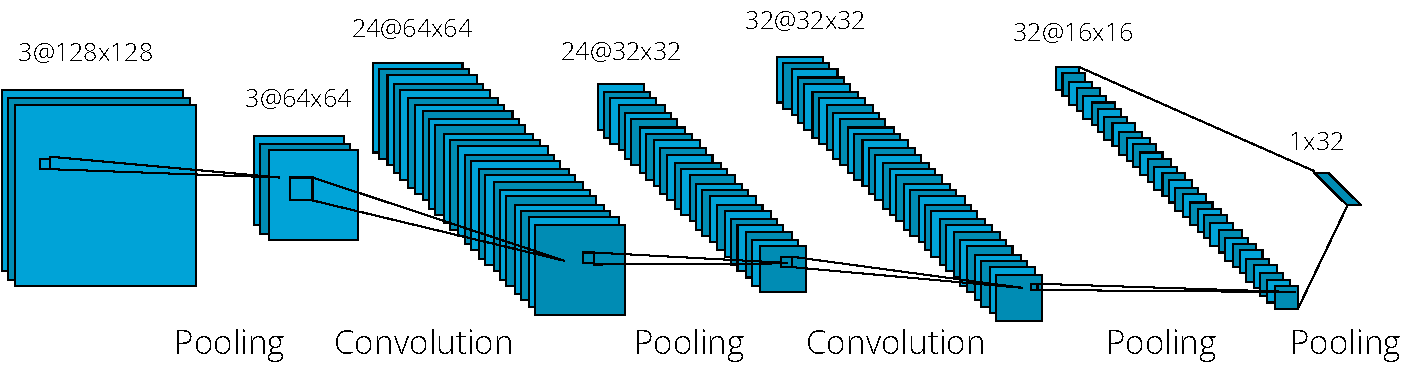
\includegraphics[width=\linewidth]{images/cnn_encoder_example.pdf}
 \caption{A typical architecture of a \ac{cnn} encoder. The encoder consists of consecutive convolutional and pooling layers that gradually increase the feature map depth and decrease its width and height. The result is a map of features that tells the decoder what features are on the image but does not provide much spatial information about the location of those features.}
 \label{fig:cnn-encoder-achitecture}
 \end{figure}

To illustrate this, we can think of a contrived example of a \ac{cnn} feature detector to detect grapes on a vine. The first few layers could do a simple operation such as edge detection, and for that, they need a lot of spatial information. The next layer could combine the edges to detect a specific shape, such as a circle. For this, it needs less spatial information as the edges are already detected. A third layer could combine several circle locations to detect a cluster of grapes on a vine. For this, it only needs a very rough location of the circles, and thus does not need detailed width and height-wise information.

A convolutional decoder can work in much the same way, but reversed. Instead of adding channels, a convolutional decoder successively removes channels and upsamples the image until the resulting image is a segmentation map $M(A) \in C \times W \times H$. Segmentation models that use only convolutional and pooling layers are called \textbf{fully convolutional models} and are one of the most widely used types of models for medical image segmentation.

\section{Commonly Used Convolutional Encoders}

Almost all medical image segmentation models employ convolutional layers in their encoder stage. 


\subsection{Balancing Inductive Bias}





